\section{Asymmetric Cryptography}
Asymmetric cryptography, also referred to as public-key cryptography, addresses the fundamental problem of symmetric cryptography in secure communications: how can two previously unknown parties establish a secure channel without first meeting up in person to exchange a secret key. 

In order to solve this problem, asymmetric cryptography uses two mathematically related keys: a private key and a public key. The public key can be distributed freely, while the private key must remain secret. Messages encrypted with a public key can then only be decrypted using its corresponding private key, enabling secure communications without the need for a predetermined shared secret.

To demonstrate this concept, imagine two people: Alice and Bob. Alice wants to send a secret message to Bob. To achieve this, they do the following: 
\begin{enumerate}
    \item Bob sends a box and an open padlock, to which only Bob has the key, to Alice.
    \item Alice places her message in the box, locks it with the padlock, and sends it back to Bob.
    \item Bob uses his key to unlock the box and is able to read Alice's message.
\end{enumerate}
Even if some adversary were to intercept the box on its way back to Bob, they would be unable to open it and read Alice's message since they don't have Bob's key.

This analogy describes the core idea of asymmetric cryptography: separating the methods of encryption and decryption. Here the padlock represents the public key, and Bob's key the private key. He can send copies of his padlock to anyone who wants to send him a secret message, knowing only he can open them.

In practice, these systems use specific mathematical problems known as trapdoor functions \cite{trapdoor}. These are problems that are easy to compute in one direction, but computationally infeasible to reverse without hidden information (the private key).

Asymmetric cryptography is not used directly to encrypt large amounts of data due to its computational overhead. Instead, it is commonly used during the initial handshake phase of a protocol to establish a shared symmetric key. Once this shared secret has been established, symmetric encryption algorithms can be used to protect the bulk of the communication efficiently.

\subsection{RSA and Diffie-Hellman}
The first generation of widely adopted asymmetric systems relied on two primary mathematical hurdles. The RSA (Rivest-Shamir-Adleman) algorithm, introduced in 1977 by Ron Rivest, Adi Shamir, and Leonard Adleman \cite{rsa}, built on the mathematical difficulty of factoring large composite integers. While multiplying two large prime numbers is computationally trivial, determining the original factors from their product is believed to be infeasible for sufficiently large numbers using classical algorithms. This asymmetry forms the mathematical foundation of the RSA algorithm.

The other fundamental primitive introduced to public-key cryptography was the Diffie-Hellman (DH) key exchange, introduced in 1976 by Whitfield Diffie and Martin Hellman \cite{dh}. Rather than encrypting messages directly, Diffie-Hellman introduced the concept of a secure key exchange, enabling two parties to establish a shared secret over an insecure channel without ever transmitting the secret itself. As illustrated in Figure \ref{fig:DH}, each party generates a private key and exchanges a corresponding public key derived from it. Both parties can then independently compute the same shared secret from the other's public key and their own private key. The security of this protocol relies on the hardness of the discrete logarithm problem, which states that recovering the private exponent from the public key alone is computationally infeasible.

\begin{figure}[H]
\centering
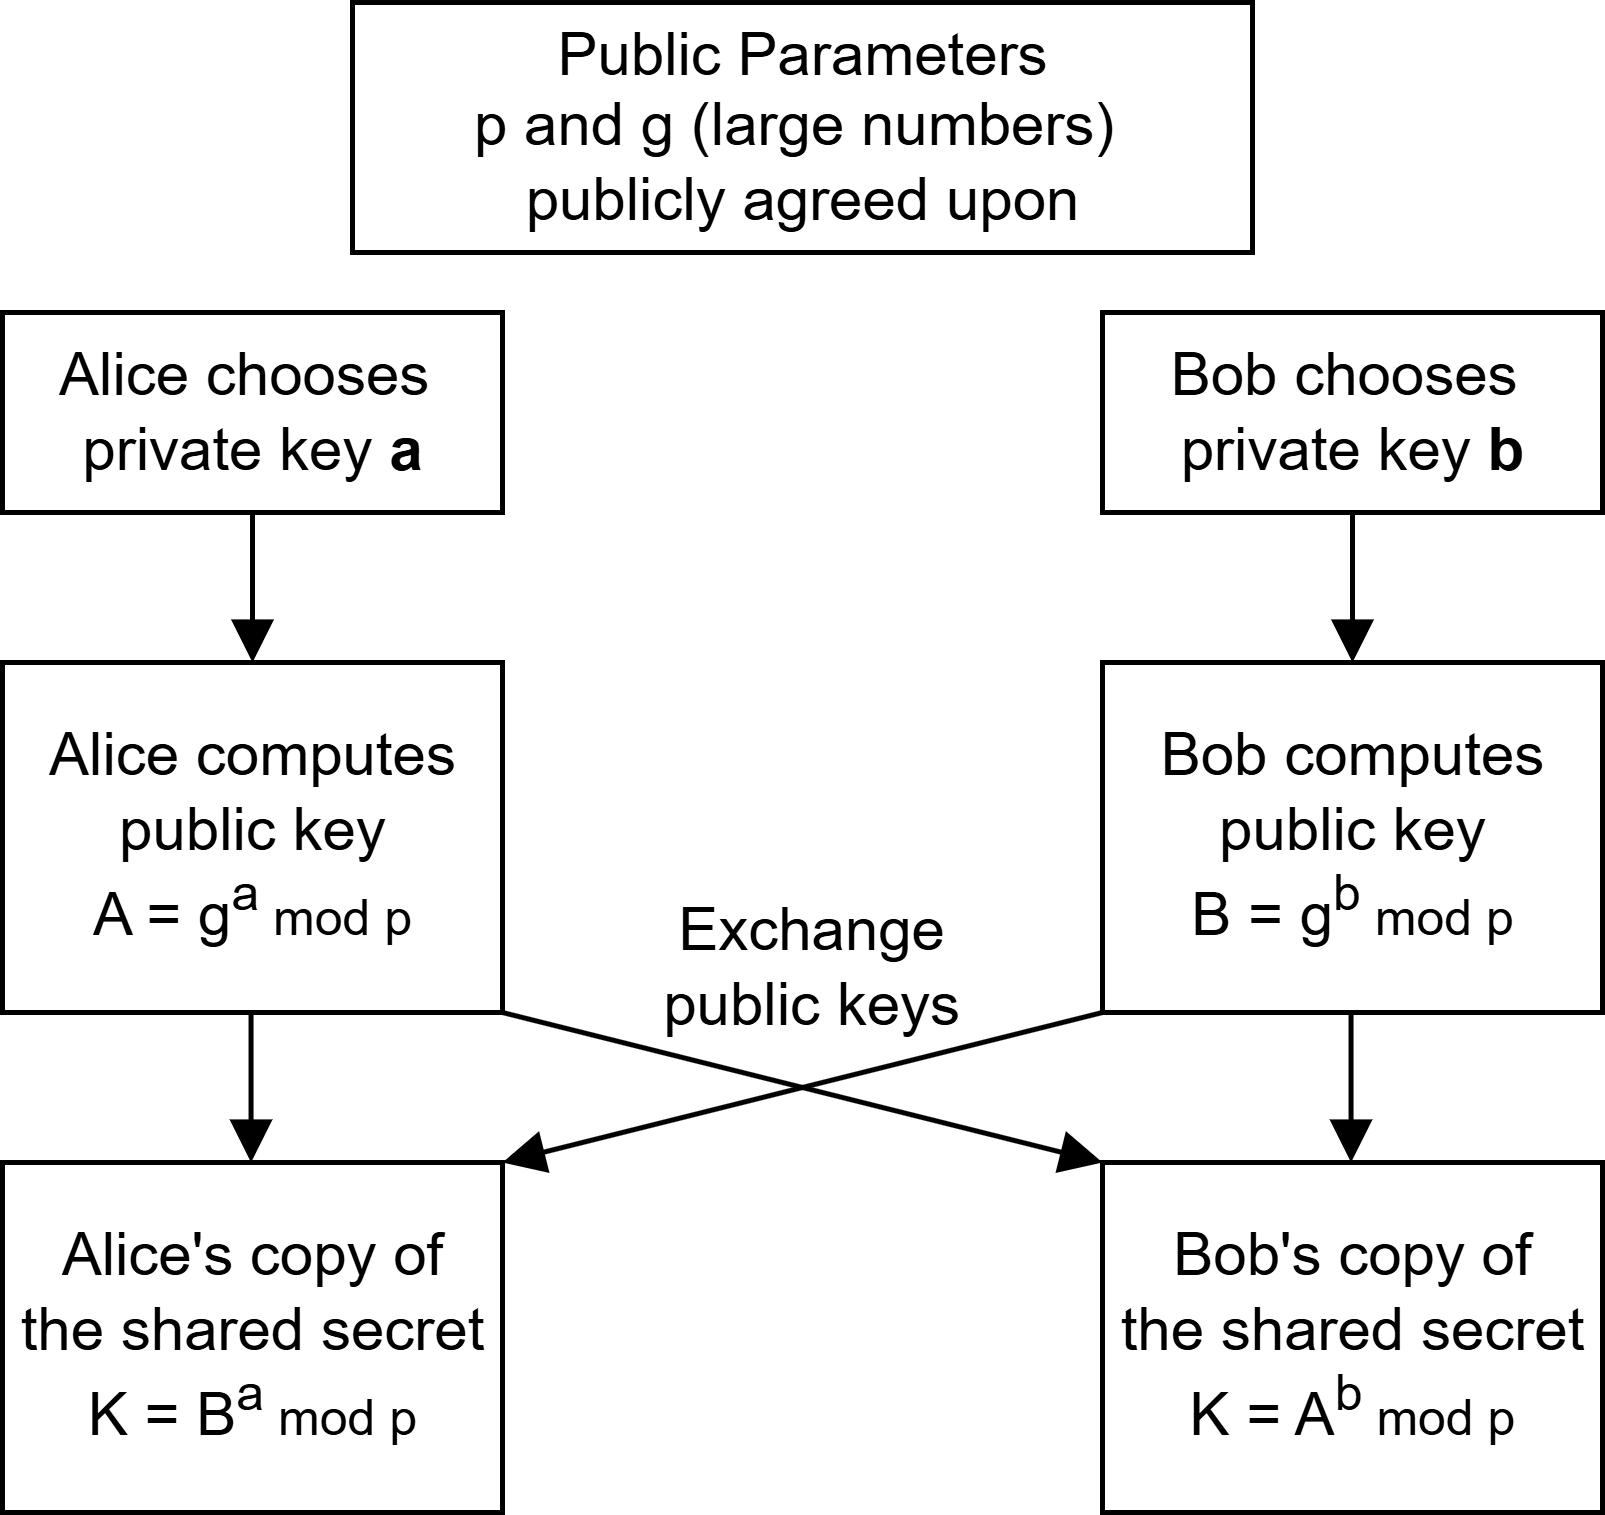
\includegraphics[width=0.8\textwidth]{Images/dh.png}
\caption{A simple view of key establishment using Diffie-Hellman.}
\label{fig:DH}
\end{figure}

These methods defined the first thirty years of digital security, but as computational power grew, the required key sizes for RSA and standard DH became unmanageable, leading to a need for more efficient mathematics.

\subsection{The Shift to Elliptic-Curve Cryptography}
In the early 2000s, many cryptographic protocols began transitioning toward Elliptic-Curve Cryptography (ECC). Instead of operating over finite fields of integers, ECC relies on the algebraic structure of elliptic curves over finite fields. The advantage of the Elliptic Curve Discrete Logarithm Problem (ECDLP) is that it is significantly harder to solve per bit of key size than the two previous mathematical problems that RSA and DH are based on.

For example, a 256-bit elliptic curve key, such as Curve25519 used by WireGuard, provides a security level equivalent to a 3072-bit RSA or DH key \cite{Barker}. This efficiency is one of the primary reasons modern protocols have adopted ECC. Smaller key sizes reduce bandwidth requirements and computational overhead, enabling faster handshakes and smaller packet headers, which are particularly important for performance-sensitive systems such as VPN protocols.

Despite their efficiency, elliptic-curve systems remain fundamentally vulnerable to quantum attacks due to their reliance on discrete logarithm problems. This vulnerability forms one of the key motivations for the development of post-quantum cryptographic algorithms. Recognizing this risk, NIST has initiated a long-term transition toward quantum-resistant cryptographic algorithms. Current guidance recommends that organizations begin migrating away from classical public-key mechanisms in the coming years, with many traditional systems expected to be phased out after approximately 2030 as post-quantum standards are deployed \cite{PQCTransition}. Such a transition highlights the need to evaluate how existing protocols that rely heavily on elliptic-curve cryptography, such as WireGuard, can adapt to post-quantum cryptographic primitives.

\subsection{Key Exchange vs. Key Encapsulation}
It's important to distinguish between the two main methods for establishing shared symmetric cryptographic keys. 

Traditional key exchange protocols such as Diffie-Hellman employ an interactive process in which both parties contribute to the generation of a shared secret. Instead of sending the secret directly, each party exchanges intermediate values derived from their private key, and both participants can independently compute the same shared key from the other's public value. This bidirectional structure is displayed in Figure \ref{fig:DH}.

In contrast, asymmetric post-quantum algorithms including ML-KEM and HQC are designed as Key Encapsulation Mechanisms (KEMs). Rather than a mutual exchange, KEMs follow a sender-receiver model. As shown in Figure \ref{fig:KEM}, the sender runs the encapsulation algorithm using the recipient's public encapsulation key, producing both a ciphertext and a shared secret. The ciphertext is transmitted to the recipient, who uses their corresponding private decapsulation key to run the decapsulation algorithm and recover the same shared secret. No interactive contribution from the recipient is required.

\begin{figure}[H]
\centering
\includegraphics[width=0.8\textwidth]{Images/kem.png}
\caption{A simple view of key establishment using a KEM}
\label{fig:KEM}
\end{figure}

While the end result is the same, both parties arrive at a shared secret, the logistical flow is different. This distinction is a core challenge when integrating post-quantum KEMs into existing protocols like WireGuard, which was originally designed for the interactive key exchange flow of Diffie-Hellman. 

Despite this difference in their structure, KEMs are the flow used for post-quantum cryptography due to the nature of the mathematical problems on which post-quantum security is based. These do not support the bidirectional structure of a key exchange protocol. Instead, they lend themselves to a one-directional approach where one party can efficiently encapsulate a secret under a public key, while only the holder of the corresponding private key can recover it.


\section{The Quantum Threat}
As discussed in the introduction, the long-term security of modern cryptographic systems relies on the assumption that certain mathematical problems are computationally infeasible for classical computers to solve. However, the development of quantum computing challenges this assumption. Quantum computers operate according to the principles of quantum mechanics and are capable of executing algorithms that can outperform classical algorithms for specific types of problems. 

There are two quantum algorithms that are especially relevant in this context: Shor's algorithm, which efficiently solves integer factorization and the discrete logarithm problem, and Grover's algorithm, which accelerates brute-force search. These algorithms are the frontrunners of the quantum threat to current cryptographic systems and are discussed in the following sections.

\subsection{Quantum Computing}
We must establish a high-level understanding of how quantum computers work in order to understand how they are able to threaten current encryption. 

A classical computer processes information using bits, binary values that exist in one of two states: 0 or 1. These bits are manipulated deterministically through electrical circuits made up of transistors and logic gates, which enables the computer to perform arithmetic and logical operations. At any given point in time, a classical system represents a single, well-defined state.

A quantum computer instead operates using quantum bits, commonly referred to as \textit{qubits}, which has the ability to exist in a superposition of both states simultaneously. As a result, a qubit represents a linear combination of the two states rather than a single deterministic value. When multiple qubits are combined, the system can represent a probability distribution of many possible states at once. For a system of $n$ qubits, this corresponds to $2^n$ possible configurations, resulting in an exponentially large state space.

The other key property of quantum systems is entanglement, where the states of multiple qubits become correlated in a way such that the state of one qubit cannot be described independently of the others. Entanglement enables quantum computers to capture and exploit relationships between variables in ways that are not possible in classical systems.

Quantum algorithms leverage superposition, entanglement, and the manipulation of probability amplitudes to perform certain classes of computations in a fundamentally different way than classical algorithms. By carefully controlling how probability amplitudes evolve during computation, these algorithms can amplify the likelihood of correct solutions while cancelling out incorrect ones. This interference structure is what enables quantum computers to achieve significant speedups over classical computation for problem classes where it can be meaningfully exploited \cite{Brassard2000Amplitude}.

\subsection{Shor's Algorithm}
One of the most significant breakthroughs in quantum computing for cryptography was the discovery of Shor's algorithm by Peter Shor in 1994 \cite{shors}. The algorithm provides an efficient quantum method for solving the two mathematical problems that are central to modern public-key cryptography: integer factorization and the discrete logarithm problem.

In order to fully grasp the impact of Shor's algorithm, let's first consider the best known classical algorithm for solving these problems. The General Number Field Sieve (GNFS) operates in sub-exponential but superpolynomial time \cite{GNFS}, which means that every additional digit in an integer makes the factorization time disproportionately longer. While significantly faster than naive approaches, the computational cost still grows at an infeasible rate for larger key sizes. The largest RSA integer factored to date is RSA-250, an 829-bit number factored in February 2020 using CADO-NFS, an optimized software implementation of GNFS \cite{CADO-NFS}. This required approximately \num{2,700} CPU core-years \cite{RSA250}, illustrating that classical factoring remains computationally prohibitive at the key sizes used in practice.

Shor's algorithm completely demolishes this notion of infeasibility. By leveraging the principles of quantum mechanics, it is able to factor large integers and solve discrete logarithms in polynomial time. It accomplishes this by reducing the problem into a period-finding problem. Given an integer $N$, the algorithm selects a random value and constructs a function whose period is related to the factors of $N$. While finding such periods is computationally difficult for classical computers, quantum computers can solve this efficiently using the Quantum Fourier Transform (QFT).

The practical implications of Shor's algorithm have been extensively explored and optimized in later research. A widely cited paper by Craig Gidney and Martin Ekerå demonstrated in 2021 that factoring a 2048-bit RSA integer could be feasible using a quantum computer with around 20 million physical qubits and 8 hours of computation time, assuming realistic error rates, cycle times and reaction times \cite{Gidney2021RSA2048}. This paper has recently received a follow-up by Gidney alone where he demonstrated that the same task could accomplished in less than a week using less than a million noisy qubits under the same assumed constraints \cite{Gidney2025RSA2048}.

Thus, the existence of Shor's algorithm represents a fundamental threat to modern public-key cryptography. Since protocols such as TLS, SSH, and VPN systems rely on RSA, Diffie-Hellman, or elliptic-curve cryptography for secure key establishment, the availability of large-scale quantum computers would render these systems insecure.

\subsection{Grover's Algorithm}
Grover's algorithm \cite{grovers} addresses a different class of problems than Shor's algorithm, specifically unstructured search. Given a search space of size $N$, a classical brute-force algorithm requires $\mathcal{O}(N)$ evaluations to find a target element. Grover's algorithm reduces this complexity to $\mathcal{O}(\sqrt{N})$ by leveraging quantum amplitude amplification.

In the context of cryptography, Grover's algorithm impacts symmetric-key primitives such as block ciphers and hash functions. But, unlike Shor's algorithm, Grover's algorithm does not completely break symmetric cryptographic schemes. Instead, it effectively halves their security level in terms of bit strength. This degradation can be mitigated by increasing key sizes. For example, a 128-bit symmetric key, which is considered secure against classical adversaries, would offer only 64 bits of security against a quantum adversary using Grover's algorithm. Consequently, doubling the key length (from 128 to 256 bits) is generally considered sufficient to maintain security in a post-quantum setting.

It is also important to note that practical implementations of Grover's algorithm face significant overhead due to error correction and circuit depth requirements, which further limits its near-term applicability. But it remains a critical consideration when evaluating the long-term security of symmetric cryptographic systems.

\subsection{``Harvest now, decrypt later.''} \label{hndl}
A common misconception about the quantum threat is that it only becomes relevant when sufficiently large quantum computers become available, but this view overlooks an already active risk model known as ``harvest now, decrypt later'' (HNDL) \cite{hndl}.

In this model, an adversary intercepts and stores encrypted communication today with the intention of decrypting them in the future once sufficiently powerful quantum computers exist. This strategy is particularly concerning for data with long-term confidentiality requirements, such as government communications, intellectual property, personal data, and critical infrastructure information. 

It is important to understand what part of modern encrypted communication is vulnerable in this context. While data at rest is protected by symmetric encryption algorithms such as AES, which are considered resistant to quantum attacks, the asymmetric public-key algorithms used during the key exchange are the primary target. If an adversary can intercept the key exchange step of a session protected by TLS for example, they can store it and later use a quantum computer to recover the symmetric session key and decrypt all the session data. The implication is that even data which appears to be well-protected at rest may be vulnerable if the key exchange that established its protection was recorded.

The HNDL threat has driven significant regulatory action across multiple jurisdictions, each establishing strict timelines for the transition to post-quantum cryptography directly motivated by HNDL risk.  

In the United States, the NSA's Commercial National Security Algorithm Suite 2.0 (CNSA 2.0) establishes a phased migration schedule for National Security Systems. Traditional networking equipment such as VPNs and routers is required to support and prefer CNSA 2.0 algorithms by 2026, and to use them exclusively by 2030. Large-scale public-key infrastructure systems, such as TLS, follow a slightly later schedule, with mandatory preference by 2030 and exclusive use by 2033 \cite{NSA2022CNSA2}. 

In Europe, the European Commission published a coordinated PQC implementation roadmap, which establishes a timeline for the transition to PQC for all member states. Under this roadmap, all member states are expected to have begun transitioning to post-quantum cryptography by the end of 2026, with critical infrastructure systems fully transitioned to PQC no later than the end of 2030 \cite{EUPQC2025Roadmap}.

At the standards level, NIST's deprecation timelines add further urgency. Classical quantum-vulnerable algorithms providing less than 128 bits of security are set to be deprecated after 2030 and disallowed after 2035, with algorithms above the 128-bit level set to follow the same eventual prohibition \cite{Moody2025PQCRoadAhead}.

The ``harvest now, decrypt later'' threat establishes that the urgency of post-quantum migration is determined not only by the arrival of quantum computers, but also by the confidentiality requirements of data being transmitted and stored today. The combination of already-active data collection, long cryptographic migration timelines, and firm regulatory deadlines means that organizations handling sensitive data must treat the transition to quantum-resistant cryptography as an active and ongoing priority.


\section{Post-Quantum Cryptography}
Post-Quantum Cryptography (PQC) refers to cryptographic algorithms that are designed to remain secure against attacks from both classical and quantum computers. The goal is to replace or complement current cryptographic primitives such as RSA, Diffie-Hellman, and ECC. In many cases, PQC schemes are designed to be integrated into existing protocols with minimal changes, although this still requires adaptations due to fundamental differences in protocol logic and accommodation for larger key sizes.

PQC algorithms are based on mathematical problems that are believed to be hard even for quantum computers. The main categories include lattice-based, code-based, multivariate, and hash-based cryptography. This thesis focuses on the two NIST-selected approaches: lattice-based cryptography (ML-KEM) and code-based cryptography (HQC).

\subsection{Lattice-Based Cryptography (ML-KEM)}
ML-KEM (Module-Lattice-Based Key-Encapsulation Mechanism), formerly known as CRYSTALS-Kyber \cite{kyber}, is a lattice-based KEM standardized by NIST in Federal Information Processing Standards (FIPS) publication 203 \cite{mlkem} in August 2024.

ML-KEM is based on the hardness of lattice problems, specifically the so-called Module Learning With Errors (MLWE) problem. The core idea is that a system of linear equations with small random errors is computationally hard to solve, even for a quantum computer.

One of the main advantages of ML-KEM is its strong performance and relatively moderate key sizes when compared to other PQC candidates. For example, ML-KEM-768 has a public key size of around \qty{1184}{bytes}, which is manageable in protocols like TLS. Key generation and encapsulation are also significantly faster than RSA. These properties make ML-KEM suitable for practical deployment, which is why NIST selected it as the primary standard for post-quantum key establishment.

\subsection{Code-Based Cryptography (Hamming Quasi-Cyclic)}
Hamming Quasi-Cyclic (HQC) \cite{hqc} is a code-based KEM selected by NIST in March 2025 as a backup standard to ML-KEM \cite{Moody2025NISTIR8545}. A draft standard is expected in 2026, with finalization planned for 2027.

The security of HQC is based on the hardness of decoding random quasi-cyclic codes, specifically the Quasi-Cyclic Syndrome Decoding (QCSD) problem. This problem is a structured variant of the general Syndrome Decoding (SD) problem, which is known to be NP-hard. Unlike older code-based schemes such as McEliece \cite{McEliece1978}, HQC does not require hiding the structure of the code. Instead, it uses publicly known quasi-cyclic codes, and its security relies entirely on the hardness of the decoding problem itself.

HQC was selected primarily to provide \textit{cryptographic diversity}. Since ML-KEM is based on lattice problems, a future cryptanalytic breakthrough targeting lattice-based cryptography could potentially affect all systems relying on ML-KEM. By standardizing HQC, which is based on a completely different mathematical foundation, NIST ensures that a backup remains available if ML-KEM is found to be vulnerable. NIST cited HQC's solid and well-analyzed construction as reasons it was preferred over other fourth-round candidates.

\subsection{Hybridization Strategies}
Because PQC algorithms are relatively new and have not yet undergone the same level of long-term cryptanalysis as classical schemes, a common deployment strategy is to combine a classical key exchange with a PQC KEM within a single handshake. This approach is known as a \textit{hybrid key exchange}.

In a hybrid scheme, a classical Diffie-Hellman exchange and a PQC KEM are executed in parallel within the same handshake. 

In the DH component, both parties contribute an ephemeral public key and independently compute the same shared secret. In the KEM component, the initiator encapsulates a secret to the responder's ephemeral public key, producing a ciphertext and a shared secret. The responder then decapsulates the ciphertext using their private key to derive the same shared secret. The two resulting secrets are then passed into a Key Derivation Function (KDF) to derive the final session key. 

The key security property of this approach is that forward secrecy is only compromised if \textit{both} components are broken. If the PQC algorithm contains an unknown vulnerability, the classical component continues to provide forward secrecy against current adversaries. Conversely, if a sufficiently powerful quantum computer becomes available in the future, the PQC component ensures that past session keys remain protected against retroactive decryption.

Hybrid key exchange is currently the industry-standard approach for deploying PQC in practice. It is already used in TLS 1.3, where hybrid mechanisms such as \texttt{X25519MLKEM768} (combining X25519 with ML-KEM-768) have been standardized by the IETF \cite{ietf-tls-ecdhe-mlkem-04}, and is being actively deployed by providers such as Cloudflare \cite{Westerbaan2025PQ}.

\subsection{Forward Secrecy}\label{sec:forward_secrecy}
Forward Secrecy (FS) is the property of a key establishment protocol where the compromise of long-term secrets used in the exchange does not expose the session keys of past communications. 

In classical protocols, FS is achieved by generating fresh ephemeral DH keypairs for each session and discarding them immediately after use. Because the session key is derived from an ephemeral secret that is never stored, a future compromise of a session key cannot be used to reconstruct past session keys.

However, as discussed in Section \ref{hndl}, classical FS alone does not protect against a quantum-capable adversary. An adversary employing the HNDL strategy can record encrypted conversations today and later break the DH exchange retroactively using a sufficiently powerful quantum computer, rendering the ephemerality of the session keys irrelevant. It is therefore necessary that Post-Quantum Forward Secrecy (PQFS) in modern cryptographic contexts is achieved using quantum-resistant primitives. 

In a hybrid key exchange, as described in the previous section, FS requires that both components contribute ephemeral keying material. Since the session key is derived from both components, one of which is a PQC KEM, PQFS holds as long as the KEM component remains secure, while the classical component continues to provide FS against non-quantum adversaries.

When PQC algorithms have withstood enough cryptanalytic scrutiny to justify sole reliance on them, it may become viable to replace the hybrid construction with a purely PQC-based key exchange. PQFS would then be achieved entirely through ephemeral KEM keypairs, with no classical component required. The security guarantees would then hold against both classical and quantum adversaries without the overhead of maintaining two parallel key exchanges.

\subsection{Practical Challenges}
PQC algorithms introduce several practical challenges that must be addressed before they can be widely deployed.

The main challenge is the significantly larger message sizes compared to classical cryptography. PQC schemes typically produce larger public keys, ciphertexts, and signatures, which increases the size of protocol messages. This can create compatibility issues with existing systems, especially older implementations that impose strict limits on message sizes. These larger key materials may require adjustments to how handshake messages are structured and transmitted.

Another challenge is the integration of PQC algorithms into existing protocols, as these were originally designed for classical key-exchange primitives and do not always directly support the encapsulate/decapsulate model of PQC schemes. As a result, careful modifications are required to assure correct functionality and maintain security guarantees. In the case of TLS 1.3, for instance, changes are needed to accommodate larger key shares and to support hybrid key exchange mechanisms.

Finally, PQC implementations must be designed with strong resistance to side-channel attacks. Like classical cryptographic algorithms, PQC schemes can leak sensitive information through timing differences, power consumption, or electromagnetic emissions. Mitigating timing-based leakage in particular requires constant-time implementations, where the execution time of cryptographic operations does not vary with secret data. Besides timing, physical side-channels also present a practical threat. Recent research has demonstrated practical chosen-ciphertext side-channel attacks against HQC implementations \cite{Goy2022HQCSideChannel}, where an adversary with physical access submits carefully crafted ciphertexts and observes electromagnetic emissions during decapsulation to fully reconstruct the secret key. The attack targets the Reed-Muller decoding step of HQC's decapsulation, and the authors propose a masking-based countermeasure as a mitigation. These findings demonstrate why careful engineering practices are critical for any real-world PQC deployment.